\documentclass[14pt,a4paper,report]{extreport}

% times new roman font
\usepackage{mathptmx}

% mock data
\usepackage{lipsum}

%russian
\usepackage[T2A]{fontenc}
\usepackage[utf8]{inputenc}
\usepackage[russian]{babel}

\linespread{1.5}

\usepackage{graphicx}

\usepackage[
    letterpaper,
    left        = 2cm,
    right       = 1cm,
    top         = 1cm,
    headheight  = 2cm
]{geometry}

%\renewcommand{\caption}{Рисунок}

\begin{document}

	\begin{titlepage}
	\begin{center}	
		\fontsize{14pt}{14pt}\selectfont
		МИНИСТЕРСТВО ОБРАЗОВАНИЯ И НАУКИ\\

		\vspace*{0.6\baselineskip}
		
		\textbf{САНКТ-ПЕТЕРБУРГСКИЙ НАЦИОНАЛЬНЫЙ ИССЛЕДОВАТЕЛЬСКИЙ УНИВЕРСИТЕТ ИНФОРМАЦИОННЫХ ТЕХНОЛОГИЙ, МЕХАНИКИ И ОПТИКИ}
		
		\vspace*{0.6\baselineskip}
		ФАКУЛЬТЕТ ИНФОКОММУНИКАЦИОННЫХ ТЕХНОЛОГИЙ
		КАФЕДРА ПРОГРАММНЫХ СИСТЕМ
	
		\vspace*{7\baselineskip}
		\fontseries{m}\fontsize{19pt}{18pt}\selectfont
		\textbf{Название типа отчета}	
		
		\fontseries{m}\fontsize{20pt}{18pt}\selectfont
		\textbf{Тема работы}\\
		\vspace*{1.15\baselineskip}
		\end{center}
	
	\vspace*{2\baselineskip}
	\begin{flushright}
	\fontseries{m}\fontsize{13pt}{10pt}\selectfont
	Выполнил Кислюк~И.~В.\\
	студент группы К4120\\
	Проверил: Преподаватель\\
	\end{flushright}
	
	\vspace*{4\baselineskip}
	\begin{center}
	Санкт-Петербург\\
	2017
	\end{center}
	
\end{titlepage}

\chapter{A chapter}
\lipsum[1]
\section{A section}
\lipsum[2]

\begin{figure}[b]
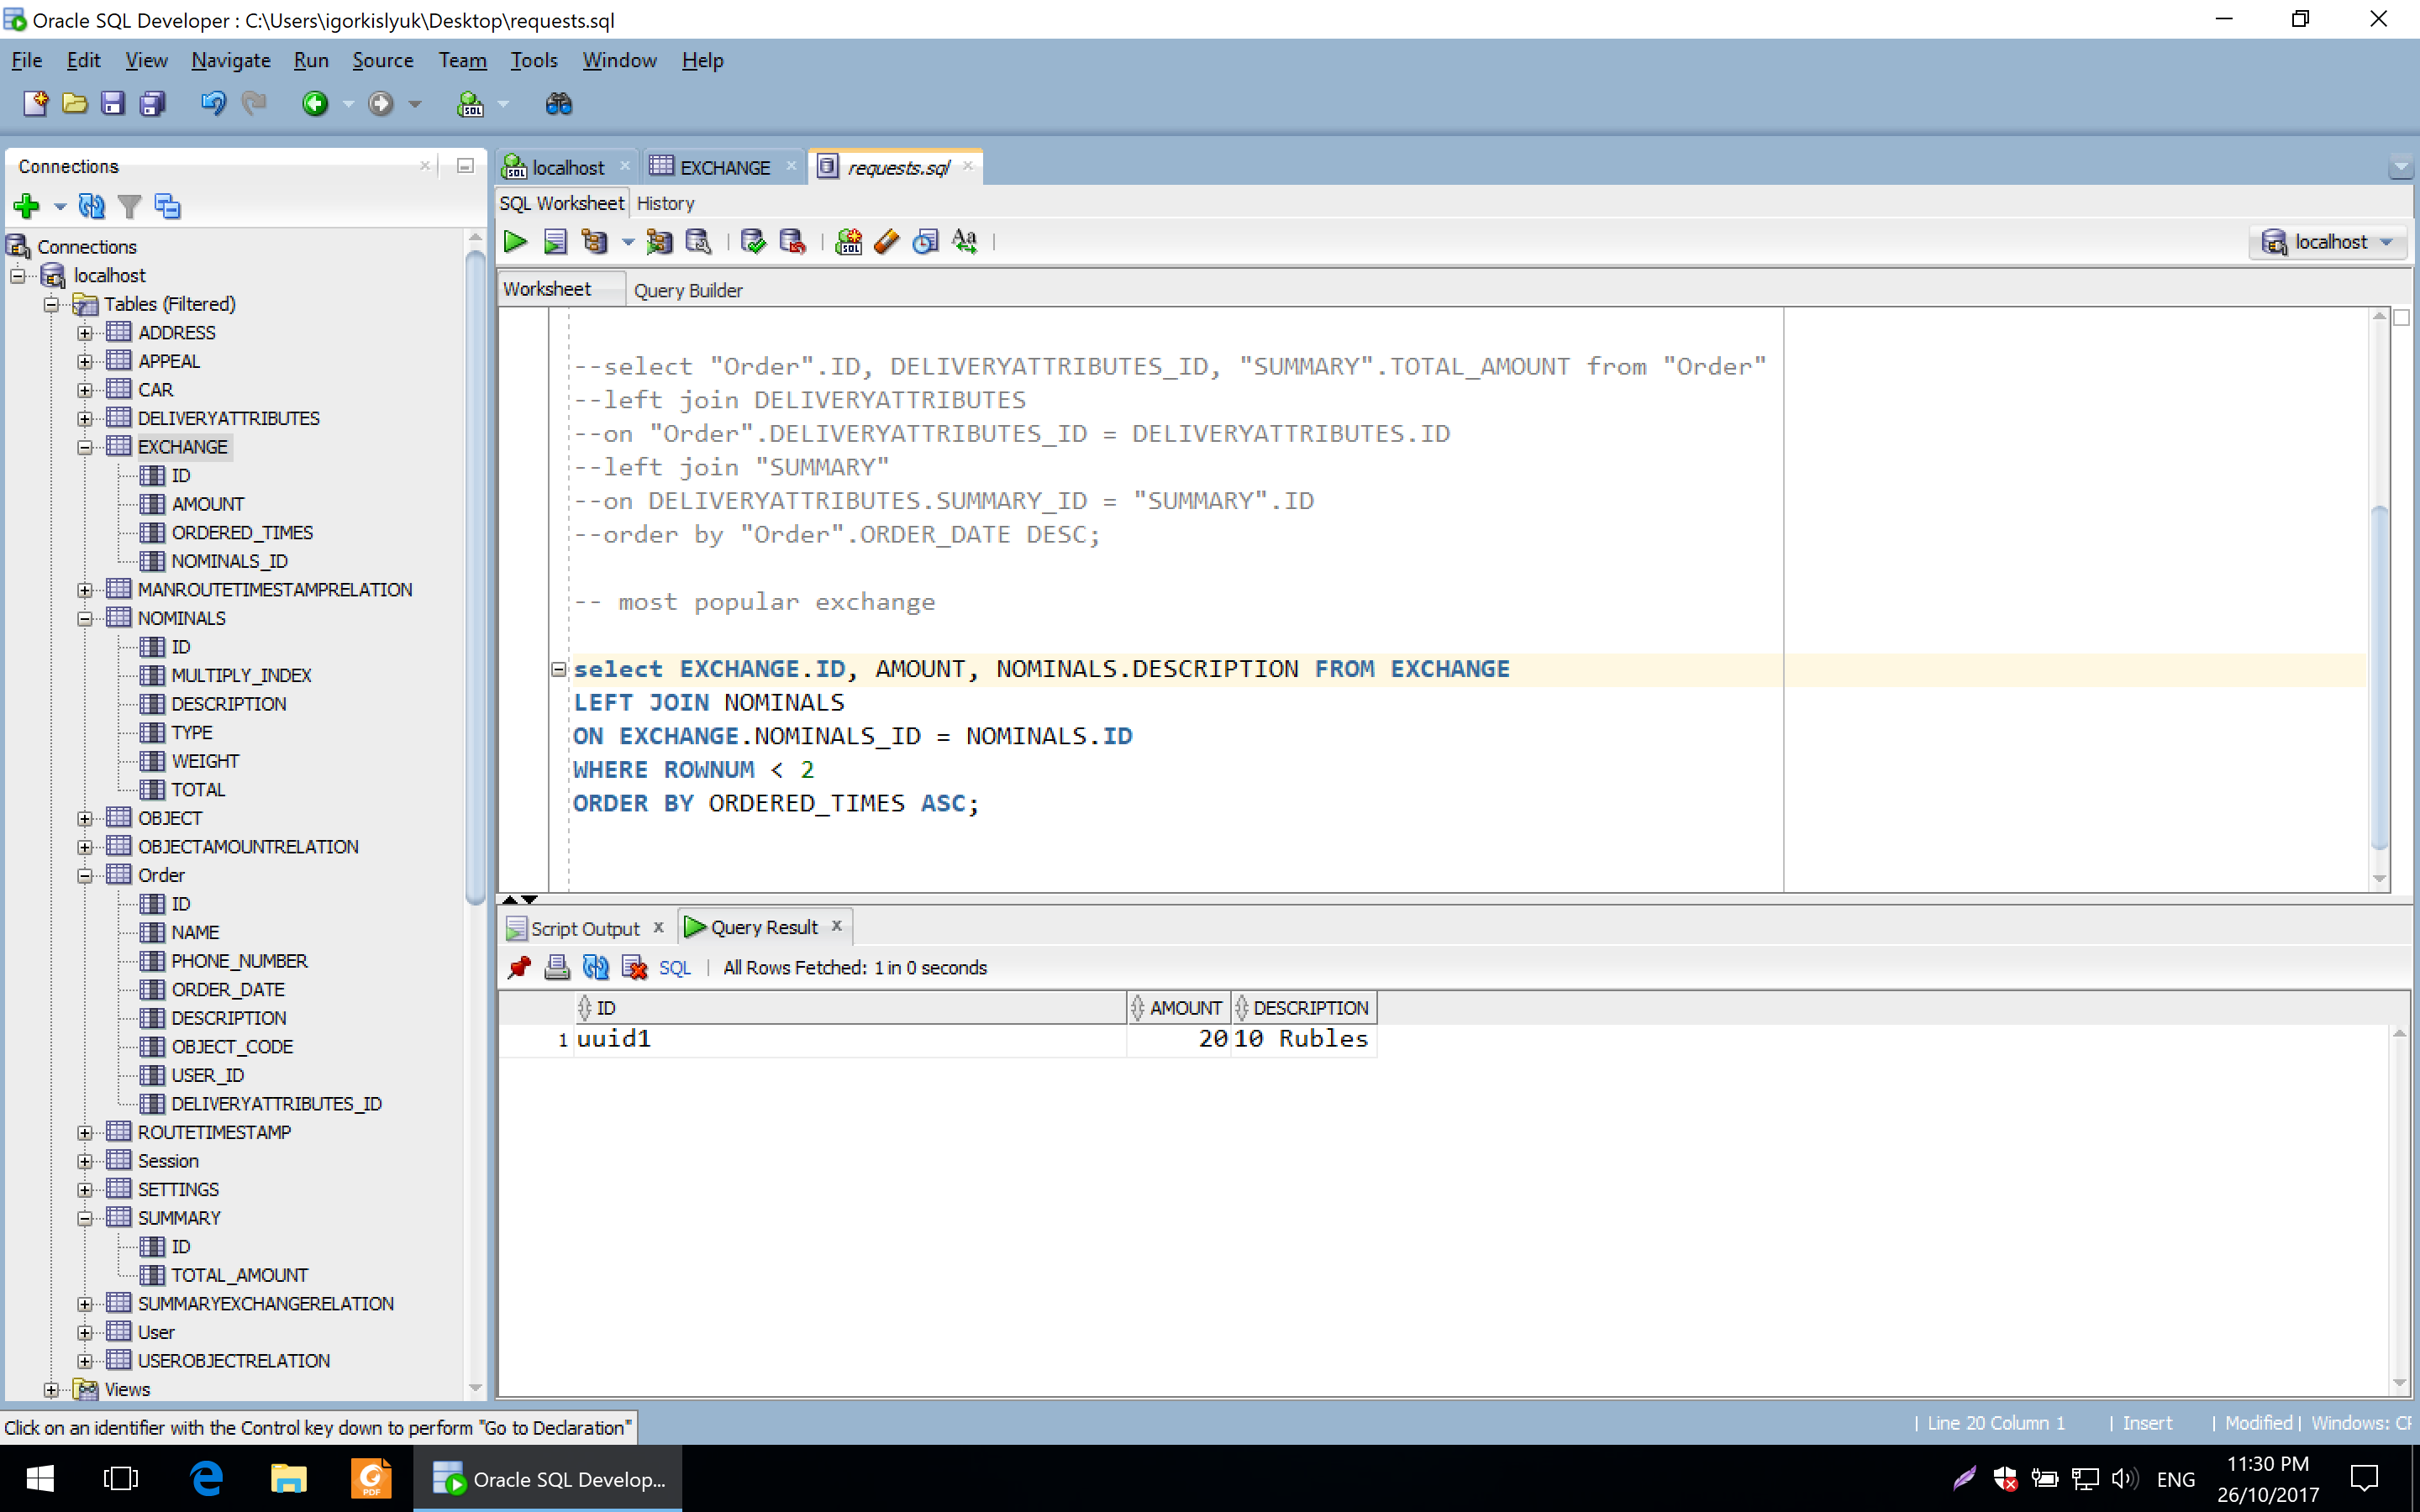
\includegraphics[scale=0.5]{image}
\caption{Рисунок}
\end{figure}

\end{document}

